% 2013 湖北卷理科第 9 题：各面涂漆的 5×5×5 正方体（TikZ 矢量重绘）。
% 以斜二测投影画出一个大正方体，并在三个可见面上画出 5×5 的分割线。
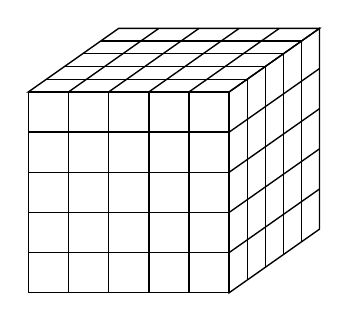
\begin{tikzpicture}[scale=0.85, line width=0.5pt, font=\small]

  \def\s{3}        % 棱长（作图单位）
  \def\dx{1.35}    % 深度方向水平分量
  \def\dy{0.95}    % 深度方向竖直分量
  \def\n{5}        % 每棱小段数
  \pgfmathsetmacro{\h}{\s/\n}

  % 前面
  \draw (0,0) -- (\s,0) -- (\s,\s) -- (0,\s) -- cycle;
  \foreach \i in {1,...,4} {
    \pgfmathsetmacro{\x}{\i*\h}
    \draw (\x,0) -- (\x,\s);
    \draw (0,\x) -- (\s,\x);
  }

  % 顶面
  \draw (0,\s) -- (\s,\s) -- (\s+\dx,\s+\dy) -- (\dx,\s+\dy) -- cycle;
  \foreach \i in {1,...,4} {
    \pgfmathsetmacro{\x}{\i*\h}
    \draw (\x,\s) -- (\x+\dx,\s+\dy);
    \draw (\x*\dx/\s,\s+\x*\dy/\s) -- (\s+\x*\dx/\s,\s+\x*\dy/\s);
  }

  % 右面
  \draw (\s,0) -- (\s+\dx,\dy) -- (\s+\dx,\s+\dy) -- (\s,\s) -- cycle;
  \foreach \i in {1,...,4} {
    \pgfmathsetmacro{\y}{\i*\h}
    \draw (\s,\y) -- (\s+\dx,\y+\dy);
    \draw (\s+\y*\dx/\s,\y*\dy/\s) -- (\s+\y*\dx/\s,\s+\y*\dy/\s);
  }

\end{tikzpicture}
